\iffalse
\documentclass[10pt,a4paper]{report}
%\usepackage[latin1]{inputenc}
\usepackage[utf8]{inputenc}
\usepackage{amsmath}
\usepackage{amsfonts}
\usepackage{amssymb}
\usepackage{graphicx}
\usepackage{multicol}
\usepackage{tabularx}
\usepackage{tikz}
\usetikzlibrary{arrows,shapes,automata,petri,positioning,calc}
\usepackage{hyperref}
\usepackage{tikz}
\usetikzlibrary{matrix,calc}
\usepackage[margin=0.5in]{geometry}
% ---- power functions -----% 
\newcommand{\myvec}[1]{\ensuremath{\begin{pmatrix}#1\end{pmatrix}}}
\let\vec\mathbf
%\providecommand $${\norm}[1]{\left\lVert#1\right\rVert}$$
\providecommand{\abs}[1]{\left\vert#1\right\vert}
\let\vec\mathbf

\newcommand{\mydet}[1]{\ensuremath{\begin{vmatrix}#1\end{vmatrix}}}
\providecommand{\brak}[1]{\ensuremath{\left(#1\right)}}
\providecommand{\lbrak}[1]{\ensuremath{\left(#1\right.}}
\providecommand{\rbrak}[1]{\ensuremath{\left.#1\right)}}
\providecommand{\sbrak}[1]{\ensuremath{{}\left[#1\right]}}
%-------end power functions----%
\newenvironment{Figure}
  {\par\medskip\noindent\minipage{\linewidth}}
  {\endminipage\par\medskip}
\begin{document}
%--------------------name & rollno-----------------------
\raggedright \textbf{Name}:\hspace{1mm} A.SUSI\hspace{3cm} \Large \textbf{Matrices Using Python}\hspace{2.5cm} % 
\normalsize \textbf{Roll No.} :\hspace{1mm} FWC22067\vspace{1cm}
\begin{multicols}{2}

%----------------problem statement--------------%

\raggedright \textbf{Problem Statement:}\vspace{2mm}
\raggedright \\
\fi
	Find the area of the circle $x^2 + y^2 = 16$ exterior to the parabola $y^2 = 6x$.\\
	\solution
	\begin{figure}[!h]
		\centering
 \includegraphics[width=\columnwidth]{chapters/12/8/3/18/figs/cp.jpg}
		\caption{}
		\label{fig:12/8/3/18}
  	\end{figure}
	\iffalse
\vspace{5mm}
%-----------------------------solution---------------------------
\raggedright \textbf{SOLUTION}:\vspace{2mm}\\

%---------given----------------%
\raggedright \textbf{Given}:\vspace{2mm}\\
Equation of circle is \\\vspace{1mm}
\begin{align}
x^2 + y^2 = 16
\end{align}
Equation of Parabola is \\ \vspace{1mm}
\begin{align}
y^2 = 6x 
\end{align}
From (2) we can say that Parabola is concave towards positive xaxis.\\ \vspace{2mm}
From equation (1) radius of circle is,\\ \vspace{1mm}
\begin{align}
r= 4
\end{align}

%-------------To find ------------------%
\textbf{To Find }\vspace{2mm}\\
To find the intersection points and area of unshaded region shown in figure\vspace{2mm}  \\ 
%--------------steps----------------------%
\textbf{STEP-1}\vspace{2mm}\\
\fi
The given circle and parabola can be expressed as conics with respectiveparameters
\begin{align}
	\vec{V}_1&=\vec{I},
\vec{u_1}=0,
f_1=-16,
\\
	\vec{V}_2&=\myvec{
0 & 0\\
0 & 1
},
\vec{u_2}= -\myvec{
3\\
0
},
f_2=0
\end{align} 
The determinant of the intersection of the given conics is 
\iffalse
\begin{align}
	\vec{x}^{\top}\brak{\vec{V}_1 + \mu\vec{V}_2}\vec{x}+2 \brak{\vec{u}_1+\mu \vec{u}_2}^{\top} \vec{x} 
	\\
	+ \brak{f_1+\mu f_2}= 0
    \end{align}
    
\begin{align}
\vec{V}_1+\mu\vec{V}_2= \myvec{
1 & 0\\
0 & \mu+1
}
\end{align}
\begin{align}
\vec{u}_1+\mu\vec{u}_2= -\myvec{
3\mu\\
0
}
\end{align}
\begin{align}
f_1+\mu f_2= -16
\end{align}
This conic is a single straight line if and only if, \\ \vspace{1mm}
\begin{align}
\mydet{\vec{V}_1 + \mu\vec{V}_2 & \vec{u}_1+\mu \vec{u}_2\\ \brak{\vec{u}_1+\mu \vec{u}_2}^{\top} & f_1 + \mu f_2} &= 0
\end{align}
And,\\
\begin{align}
\mydet{\vec{V}_1 + \mu\vec{V}_2} &= 0
\end{align}
Substituting equation (13),(14) and (15) in equation (16)\\ \vspace{1mm}
We get,\\ \vspace{1mm}
\fi
\begin{align}
\implies \mydet{1& 0 & -3\mu\\ 
0 & 1+\mu & 0 \\
-3\mu & 0 & -16
} &= 0
\end{align}
yielding
\begin{align}
	9\mu^3 + 9\mu^2 + 16\mu + 16&=0
	\\
	\text{or, }
    \mu = -1
\end{align}
\iffalse
 Thus, the parameters for a straight line can be expressed as\\ \vspace{1mm}
 \begin{align}
	\vec{V} &= 
\vec{V}_1 + \mu\vec{V}_2
=\myvec{ 1 & 0 \\ 0 & 0},
\\
	\vec{u} &=
\vec{u}_1+\mu \vec{u}_2
	= \myvec{
-3\\
0
    }
\\
	f&=-16,
	\\
	\implies \vec{D} &= \vec{V}, \vec{P} = \vec{I}
    \end{align}
 

with the conic section 
\begin{align}
	\vec{x}^{\top}\vec{V}\vec{x} + 2\vec{u}^{\top} \vec{x} + f = 0
\label{eq:conic_quad_form}
\end{align}
\begin{align}
    \myvec{x & y}\myvec{
1 & 0\\
0 & 0I
}\myvec{x \\ y}+2\myvec{-3 & 0}\myvec{x\\y}-16=0
\end{align}\begin{align}
   q=\myvec{2\\-8} 
\end{align}
\noindent Thus, the desired pair of straight lines are \\
\begin{align} 
	\myvec{2 \\-8 }x+ \myvec{0 &1}y
	\\
\end{align} 
upon substituting from  The points of intersection of the line 
\begin{align}
L: \quad \vec{x} = \vec{q} + \kappa \vec{m} \quad \kappa \in \mathbb{R}
\label{eq:conic_tangent}
\end{align}
\begin{align}
\vec{x}_i = \vec{q} + \kappa_i \vec{m}
\label{eq:conic_tangent_pts}
\end{align}

\begin{align}
\noindent with the conic section  we have ,
\end{align}
\begin{align}
\vec{x}_i = \vec{q} + \kappa_i \vec{m}
\end{align}
where, \\
{\tiny
\begin{multline}
\kappa_i = \frac{1}
{
\vec{m}^T\vec{V}\vec{m}
}
\lbrak{-\vec{m}^T\brak{\vec{V}\vec{q}+\vec{u}}}
\\
\pm
\rbrak{\sqrt{
\sbrak{
\vec{m}^T\brak{\vec{V}\vec{q}+\vec{u}}
}^2
-
\brak
{
\vec{q}^T\vec{V}\vec{q} + 2\vec{u}^T\vec{q} +f
}
\brak{\vec{m}^T\vec{V}\vec{m}}
}
}
\end{multline}
}
On substituting\\
\begin{align}
\vec{q} &= \myvec{
2\\
-8
} 
\end{align}
\begin{align}
\vec{m} = \myvec{0 \\ 1}
\end{align}
With the given circle\\ 
\begin{align}
	\vec{V} &= \myvec{
1 & 0\\
0 & 1
    }
\end{align}
\begin{align}
	\vec{u} = -\myvec{0 \\0}
 \end{align}
 \begin{align}
  f = -16
 \end{align}
The value of q ,\\
\begin{align}
    q = 2,-8
\end{align}
The points of intersection with Parabola along circle are \\
\begin{align}
    \vec{A}=\myvec{
2\\
3.46
    }
\end{align}
\begin{align}
    \vec{B}=\myvec{
2\\
-3.46
    }
\end{align}
\textbf{Result}
\begin{center}
\begin{minipage}[b]{0.4\textwidth}
    \includegraphics[scale = 0.4]{cp.jpg}
  \end{minipage}
\end{center}\vspace{1mm}
 From the figure,\\ \vspace{1mm}
Total area of circle exterior to the parabola is given by, \\ \vspace{1mm}
A=Area of circle-2[Area(OAD)+Area(DAC)]
\begin{align}
 B=  \int_{0}^{2} y \,dx+\int_{2}^{4}y \,dx 
\end{align}
\begin{align}
 B=  \int_{0}^{2} f(x) \,dx+\int_{2}^{4} g(x)\,dx 
 \end{align}
 Where g(x) is area of circle and f(x) is the area of parabola around the points\\ \vspace{1mm}
\begin{align}
B= \int_{0}^{2} {\sqrt{16 x}}\,dx + \int_{2}^{4} {\sqrt{16-x^2}}\,dx 
\end{align}
\begin{align}
B=\frac{4}{3}(4\pi+\sqrt{3})\\
\end{align}
Area of circle\\
\begin{align}
C= \pi×(r^2)\,dx
\end{align}
\begin{align}
C= \pi×(4^2)\,dx=16\pi
\end{align}
\begin{align}
A= C-B
\end{align}
Area A is,\\ 
\begin{align}
    A= 16\pi-\frac{4}{3}(4\pi+\sqrt{3}) \,m^2
\end{align}
\begin{align}
    A= 31.200 \,square units
\end{align}

 \vspace{2mm} \textbf{Construction}
\begin{center}
\setlength{\arrayrulewidth}{0.5mm}
\setlength{\tabcolsep}{6pt}
\renewcommand{\arraystretch}{1.5}
    \begin{tabular}{|l|c|}
    \hline 
    \textbf{Points} & \textbf{coordinates} \\ \hline
   $\vec{A}$ & $\myvec{
   2\\
   3.46
   } $ \\\hline
   $\vec{B}$ & $\myvec{
   2\\
   -3.46
   } $ \\\hline
      \end{tabular}
  \end{center}

*Verify the above proofs in the following code.\\
\framebox{
\url{https://github.com/Susi9121/FWC/tree/main/matrix/line}}	
\bibliographystyle{ieeetr}
 \end{multicols}
\end{document}
\fi
